\documentclass[12pt]{article}

\usepackage{fontawesome}
\usepackage{hyperref}
\usepackage{xurl}
\usepackage{graphicx}



\hypersetup{
    colorlinks=false,
    pdfborder={0 0 0},
}


\title{SQL Challenges}
\author{
        Adrianna Holden-Gouveia \\
        Website: \url{https://aholdengouveia.name}\\ 
        \date{\vspace{-5ex}}
        %Email: \href{mailto:admin@aholdengouveia.name}{admin@aholdengouveia.name} \\
        \faLinkedin{: aholdengouveia} \\
        \faGithub {: aholdengouveia} \\
        %\faTwitter {: aholdengouveia} \\
        }

%S\date{\today}


\begin{document}    

\maketitle

%\begin{abstract}
%This is a template for Linux Administration Lab work
%\end{abstract}
%\tableofcontents

\section*{Objectives:}
\begin{itemize}
    \item The objective of this lab is to work on challenges for SQL problem solving. Prior knowledge SQL is assumed. Students will attempt more real world applications of SQL on interactive methods utilizing a free online tutorial and other resources.
\end{itemize}
\section*{Instructions}

References, a video, a PowerPoint and some notes are available at my website
\url {https://www.aholdengouveia.name/IntroData/sql3.html}

The challenges are here: \url{https://www.hackerrank.com/domains/sql} You will need to register, but it's a free site. 


\textbf{You must do at least 10 basic/easy and 1 intermediate/medium (or advanced) challenge, make sure to number each challenge and label if it's the basic/easy or the intermediate/medium}

\subsection*{Please include answers to the following questions}

There is a document that should be used called SQLchallenges.docx which has an example of what your answers should look like, you can use that as a base for your deliverable.
    \begin{enumerate}
        \item For each challenge explain the query you used to solve the problem in your own words.
        \item What resources did you need for these challenge(s)?
        \item Rate the difficulty of each challenge on a scale of 1 (easy) to 10 (hard) and explain why you gave it the rating you did.
        \item Would you recommend the challenge to others? 
        \item Take screenshots of the solution to each challenge. Make sure to have a note with your name and the term in the screenshot, screenshot should be focused on the note and answer, not the full desktop.  Any screenshots that don't include the note, or are full desktop, or taken with a camera instead of a screenshot won't count and will earn no points. This is an example of what it should look like:        
 
        \begin{figure}[h!]
            \centerline{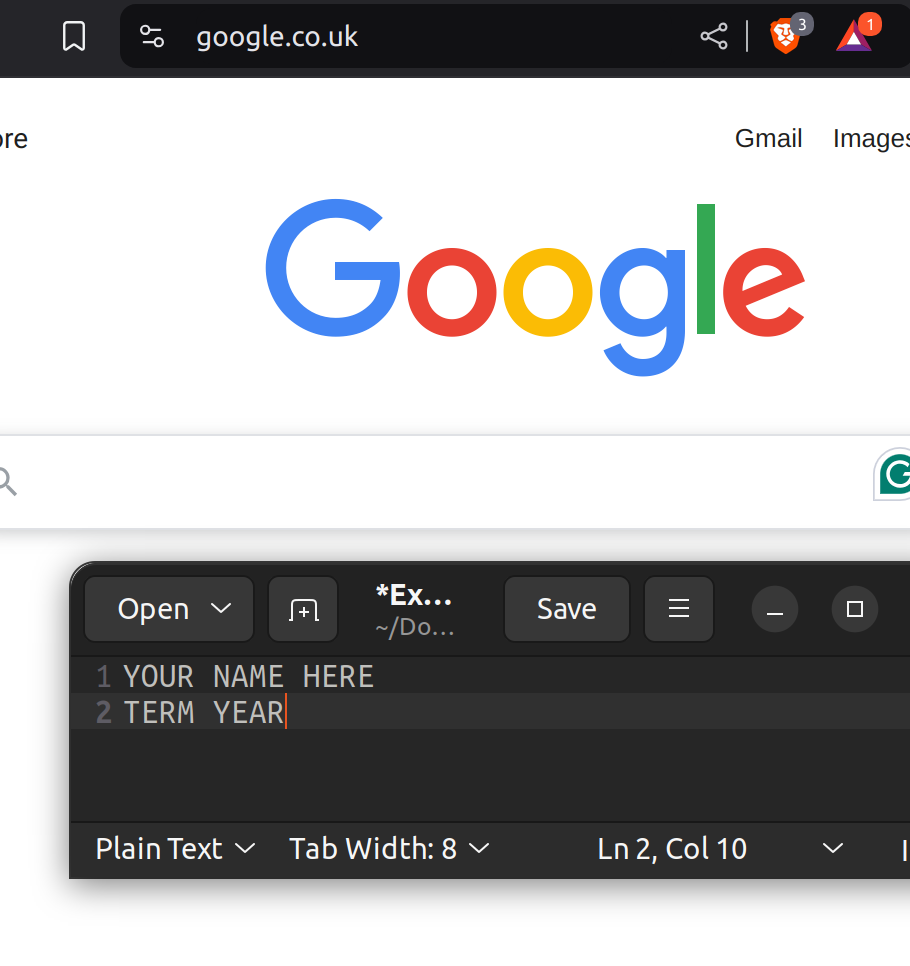
\includegraphics[scale=.2]{ExampleScreenshot.png}}
            \caption{This is an image of what each of your screenshots should look like}

            \end{figure} 
    \end{enumerate}


\section*{Deliverables:}
\begin{itemize}
    \item Answers to the above question and all requested screenshots in the format given on the SQLchallenges.docx
    \item A screenshot of your HackerRank Profile that shows the SQL badge and your username.  Make sure this screenshot follows the requested format with your name and the term.
    \item This should be a single file submitted, with everything clearly labelled.
\end{itemize} 
\end{document}